\documentclass{llncs}

\usepackage[usenames]{color} 
% \newcommand{\editIns}[1]{#1}
\newcommand{\editIns}[1]{\textcolor{red}{#1}}
% \newcommand{\editDel}[1]{\textcolor{blue}{#1}}
\newcommand{\editDel}[1]{}

\usepackage[cmex10]{amsmath}
\usepackage{amssymb}

\usepackage{paralist}

\usepackage[compress,sort]{cite}
\usepackage{hyperref}
\usepackage{url}
\hyphenation{}

\usepackage{caption}%[caption=false]{caption}
\usepackage[font=footnotesize]{subcaption}
% \usepackage[tight,footnotesize]{subfigure}
% \usepackage{fixltx2e}
% \usepackage{stfloats}
%% \usepackage[caption=false,font=footnotesize]{subfig}
\usepackage{booktabs}

\usepackage[linesnumbered,vlined,boxed]{algorithm2e}%ruled,
\usepackage{blockmatrgraph}


\usepackage{xspace}
\newcommand{\MKL}{{\sc MKL}\xspace}
\newcommand{\Blas}{{\sc BLAS}\xspace}
\newcommand{\Lapack}{{\sc LAPack}\xspace}
\newcommand{\Plasma}{{\sc Plasma}\xspace}

\newcommand{\Cuda}{{\sc CUDA}\xspace}
\newcommand{\CuBlas}{{\sc Cu\Blas}\xspace}
\newcommand{\CuSparse}{{\sc CuSPARSE}\xspace}

\newcommand{\Magma}{{\sc Magma}\xspace}
\newcommand{\Cula}{{\sc CuLA}\xspace}
\newcommand{\PhiGemm}{{\sc PhiGEMM}\xspace}
\newcommand{\Paralution}{{\sc Paralution}\xspace}
\newcommand{\Cusp}{{\sc CUSP}\xspace}
\newcommand{\Quest}{{\sc QUEST}\xspace}

\newcommand{\Bsof}{\texttt{BSOF}\xspace}
\newcommand{\Bstri}{\texttt{BSTRI}\xspace}
\newcommand{\Bsoftri}{\texttt{BSOFTRI}\xspace}
\newcommand{\Bsoi}{\texttt{BSOI}\xspace}
\newcommand{\Gemm}{\texttt{DGEMM}\xspace}
\newcommand{\Trmm}{\texttt{DTRMM}\xspace}
\newcommand{\Trsm}{\texttt{DTRSM}\xspace}
\newcommand{\Lacpy}{\texttt{DLACPY}\xspace}
\newcommand{\Trtri}{\texttt{DTRTRI}\xspace}
\newcommand{\Geqrf}{\texttt{DGEQRF}\xspace}
\newcommand{\Orgqr}{\texttt{DORGQR}\xspace}
\newcommand{\Ormqr}{\texttt{DORMQR}\xspace}
\newcommand{\Ilaenv}{\texttt{ILAENV}\xspace}


\begin{document}
\title{
  Structured Orthogonal Inversion of Block $p$-Cyclic Matrices 
  on Multicores with GPU Accelerators
\thanks{
This work was supported by the National Science Foundation 
under grant NSF-PHY-1005503. SG would like to thank the Fulbright 
Program Office in Ukraine and the Institute of International Education 
for financial support during this study.
This research used resources of the National Energy Research
Scientific Computing Center, which is supported by the Office of
Science of the U.S. Department of Energy under 
Contract No. DE-AC02-05CH11231.}
}
\titlerunning{BSOI on Multicores with GPUs} 

\author{Sergiy Gogolenko\inst{1} 
  \and Zhaojun Bai\inst{2}
  \and Richard Scalettar \inst{2}}
\authorrunning{S. Gogolenko, Z. Bai, and R. Scalettar}
\tocauthor{Sergiy Gogolenko, Zhaojun Bai, Richard Scalettar}

\institute{%Department of Computer Engineering, 
  Donetsk National Technical University, 
  Donetsk, 83001, Ukraine\\
  \email{sergiy.gogolenko@gmail.com}
  % \\ WWW home page: \url{http://ki.donntu.edu.ua/~gogolenko/}%\homedir
  \and % Department of Computer Science, 
  University of California, 
  Davis, CA 95616, USA \\
  \email{\{bai@cs,scalettar@physics\}.ucdavis.edu}}

\maketitle


\begin{abstract}
%  Block $p$-cyclic matrices are an important class of block structured
%  matrices with broad applications such as 
%  numerical solutions of differential equations, 
%  Markov chain modeling, 
%  and quantum Monte Carlo simulations. 
%  The explicit inversion of the block $p$-cyclic matrices is 
%  a common computational kernel in these applications.
  % It is well known that the standard Gaussian
  % elimination with partial pivoting based algorithms could be numerically
  % unstable. In contrast, orthogonal factorization based methods are
  % numerically stable but require more floating point operations.
%In this paper, 
We present a block structured orthogonal factorization (BSOF) algorithm
and its parallelization for computing the inversion of block $p$-cyclic matrices. 
We aim at the high performance on multicores with GPU accelerators. 
We provide a quantitative performance model for optimal host-device 
load balance, and validate the model through numerical tests.
Benchmarking results show that the parallel BSOF
based inversion algorithm attains up to 90\% of 
{\tt DGEMM} performance on hybrid CPU+GPU systems.

\begin{keywords}  
$p$-cyclic matrix; matrix inversion; 
structured orthogonal factorization;
    % load balancing; 
performance modelling; 
GPU acceleration%; \Cuda multi-GPU programming
  \end{keywords}
\end{abstract}


\section{Introduction}

Since the pioneering works of
Varga, Young, Romanovsky, and others in the 1950s, % \cite{Varga59,Varga09}, 
$p$-cyclic matrices
have been found to be a very useful class of structured matrices
with applications in numerical solutions of differential equations, 
Markov chain modeling and quantum Monte Carlo simulations. 
The concept of block $p$-cyclic matrices
in its modern term refers to matrices which can be
transformed to the following \emph{normalized block $p$-cyclic form} 
by row and/or column permutations: 
\begin{equation} \label{eq:matr_A}
  H =
  \begin{bmatrix}
    A_1 &    &    &  & B_p   \\
    B_1 & A_2 &    &  &  \\
        & B_2 & A_3 &  &     \\
            &        & \ddots & \ddots &         \\
        &     &          & B_{p-1} & A_p
  \end{bmatrix}
  ,
\end{equation}
where $A_i$ and $B_i$ are non-zero blocks.
For the sake of simplicity, in this paper,
we are concerned entirely with the {normalized block $p$-cyclic matrices},
and furthermore, we assume that 
$A_i$ and $B_i$ are $n$-by-$n$ square blocks, although
in some applications $A_i$ and $B_i$ are rectangular.
The fact that we discuss only matrices with the square blocks $A_i$ and $B_i$
does not limit the generality of approaches presented in this paper.

The early studies of $p$-cyclic matrices 
were closely related to numerical solution of differential 
equations~\cite{Wright93,Wright92BSOF,Fairweather04}.
In these applications, the $p$-cyclic matrices are also 
referred to as bordered almost block diagonal 
(BABD) matrices.  An incomplete list of 
BABD-based numerical algorithms includes multiple shooting 
and finite difference schemes for two-point boundary value problems (BVPs),
orthogonal spline collocation methods for separable elliptic BVPs, 
method of lines and Keller's box scheme for various initial 
BVPs~\cite{Wright92BSOF,Fairweather04}.
%
The $p$-cyclic matrices also appear in 
Markov chain modeling, where the $p$-cyclic stochastic 
matrices represent infinitesimal generators of continuous-time 
Markov chains with periodic transition graphs for queuing networks 
and stochastic Petri nets~\cite{Ernst00}. %~\cite{Stewart94,Niethammer00,Marek03}.
%
In quantum Monte Carlo (QMC) simulations of Hubbard models for
strongly correlated materials,
the inverses of $p$-cyclic matrices, referred to as Green's functions, 
are required to be repeatedly computed {\em explicitly} for 
physical observables, see~\cite{Bai09,Tomas12} and references therein. %Loh92,@TODO
Other sources of applications of $p$-cyclic matrices include
some linear least-square problems and parameter estimation with 
non-linear differential algebraic equations (DAE) models.

In contrast to the subject of solving block $p$-cyclic linear systems, 
where we observe tremendous progress over the last six decades,
the problem of computing $p$-cyclic matrix inversion explicitly remains in 
a state of infancy. The recent advances are mainly related to 
computing some particular blocks in the inverse of a $p$-cyclic matrix
using well-known explicit expressions~\cite{Bai09,Tomas12}.
For instance, the paper~\cite{Tomas12} addresses stabilized algorithms for 
calculation of diagonal blocks of the inverse of block $p$-cyclic matrices. 
To the best of our knowledge, there is no previous work 
focused on numerical algorithms for the entire inversion of 
block $p$-cyclic matrices, which is required for 
time-dependent physical measurements in the quantum Monte Carlo 
simulation~\cite{Bai09}.
Filling this gap is the main purpose of our paper. 
% We explore the potential of conventional way for numerical inversion 
% of matrices, where the matrix factorization is an inevitable first step in 
% preparation to computing inverse itself. %~\cite{GolubVanLoan13}. 
% Taking into account results on 
% the numerical stability and robustness of direct solvers 
% for $p$-cyclic linear systems,
% we develop a structured orthogonal factorization (SOF) based inversion algorithm 
% in place of the conventional pivoted LU factorization based approach.

In this paper, we pay particular attention to 
algorithmic solutions designed specifically for high performance computing 
on GPU accelerated multicore systems.
We should point out that numerical libraries for GPGPU computing,
including widely used 
\CuSparse, % ~\cite{CuSparse13}, 
\Cula, %~\cite{Humphrey10CULA}, 
\Paralution, %~\cite{Paralution13}, 
and \Cusp, % ~\cite{CuspLib13},
do not support inversion of structured %% and sparse 
matrices.
Furthermore, solvers in dense linear algebra libraries for GPUs 
such as \CuBlas, %~\cite{CuBlas13}
\Magma~\cite{Tomov10Magma}, %Agullo09,
and \Cula, %~\cite{Humphrey10CULA}, 
do not implement mechanisms for avoiding redundant 
computations with zero-blocks.

\section{Previous work} 
\label{sec:background}

Historically, the studies of $p$-cyclic matrices
were primarily focused on iterative and direct methods for 
$p$-cyclic linear systems. The vast literature on iterative methods 
covers in detail successive overrelaxation,
aggregation and disaggregation,
Chebyshev semi-iterative, 
and Krylov subspace methods~\cite{Ernst00}.
% including preconditioned conjugate gradients~\cite{Amodio00}, 
On the other hand, the attention to the direct solvers 
is also remarkable.
Researchers explored numerous variations of Gaussian elimination and 
orthogonal factorization approaches for solving $p$-cyclic systems.
There is a large volume of literature on Gaussian elimination
dealing with a special case of $p$-cyclic systems, 
called almost block diagonal (ABD) systems~\cite{Wright92BSOF}.
Nevertheless, while 
handling % tending to handle 
the ABD systems successfully, 
Gaussian elimination processes could fail.
In fact, in~\cite{Wright93}, it is shown that 
the Gaussian elimination with row partial pivoting %(GEPP)
produces exponential error growth
for $p$-cyclic systems arising from multiple shooting for 
some linear BVPs with mixed two-point boundary conditions. 
There is a number of approaches that enlarge the class of linear systems
for which numerical stability is ensured, 
such as certain forms of pre-scaling
and replacing row-by-row pivoting with 
more accurate panel pivoting strategies.
In the recent paper~\cite{KhabouDGG13} Khabou et al.
propose to use a panel rank-revealing pivoting strategy 
based on strong rank revealing QR, 
which significantly reduces the growth factor, and 
thus results in practical stability of Gaussian elimination
in most cases.

Due to numerical stability issues of Gaussian elimination algorithms, 
Wright proposed to use a structured orthogonal 
factorization (SOF)~\cite{Wright92BSOF}.
He described a serial and two parallel block SOF algorithms. 
The first parallel algorithm uses the recursive factorization 
process similar to cyclic reduction,
whereas the second one factorizes $p$-cyclic matrix in two steps,
at first splitting the entire matrix in parts and factorizing these 
parts concurrently, and then performing factorization of the reduced 
$p$-cyclic matrix formed from border blocks of the parts factorized 
in the previous step.  A proof of the stability of 
SOF is presented in \cite{Wright92BSOF}.
% \editDel{On the other hand, Jackson and Pancer proposed 
% another stable structure-exploiting orthogonal factorization 
% procedure for $p$-cyclic systems. It is referred to as 
% a stable local orthogonal factorization (SLF-QR) algorithm~\cite{Jackson92}.}

\section{Basic algorithms}
\label{sec:algorithm}

This section gives a brief overview of an algorithm for 
structure-exploiting orthogonal inversion 
of block $p$-cyclic matrices. It is referred to as BSOFI. 
For more details of the BSOFI and its modifications such as blocking and batching, 
we refer readers to our technical report~\cite{GogolenkoBai13}.

The algorithmic framework of BSOFI is composed of three phases. 
The first one is the block SOF of $H$: $H = QR$.
Once factors $Q$ and $R$ are computed, 
the inverse is calculated by the identity $H^{-1} = R^{-1}Q^T$
in two phases, namely inversion of the factor $R$ 
and applying the transpose of the factor $Q$.
%Our inversion algorithm appears to be backward stable,
%inheriting this property from its core operations, 
%namely Householder transformation and block back substitution, 
%which are well known to have backward stability.

\textit{Block structured orthogonal factorization (BSOF)} 
is a block structured QR factorization algorithm introduced 
in~\cite{Wright92BSOF}, and has an identical complexity to the best known 
block structured Gaussian elimination based algorithm. 
The essence of this algorithm is 
in transformation of the matrix $H$ 
through a sequence of $p-1$ block row updates (Fig.\,\ref{alg:BSOF}). 
\editDel{In the $k$th step, we treat $k$th and $(k+1)$th block rows of $H$.
At first, we perform the QR factorization of 
$2n$ by $n$ submatrix $[\tilde{A}_k^T, B_k^T]^T$ 
using Householder reflectors 
and then we apply the computed Householder reflectors from left 
in the reversed order to the selected non-zero block columns of the rows. }

\begin{figure}[t]  
\centering 
\begin{algorithm}[H]%[thb]
  %\footnotesize % \scriptsize

  \KwData{$H$, $n$, $p$}
  \KwResult{$R$, $\{Q^{(k)} | 1 \leq k < p - 1 \}$}
  \BlankLine

  $R \gets O$; $\tilde{A}_1 \gets A_1$ ; $\tilde{B}_1 \gets B_p$\; 

  \For{$k \in \{1, 2,..., p-2 \}$ }{
    Compute regular QR: 
    $Q^{(k)} 
    \begin{bmatrix}
      R_{kk} \\ 0
    \end{bmatrix}
    =
    \begin{bmatrix}
      \tilde{A}_k \\ B_k
    \end{bmatrix}$\;

    %% Update 
    $\begin{bmatrix}
      R_{k,k+1} & R_{k,p} \\ \tilde{A}_{k + 1} & \tilde{B}_{k + 1}
    \end{bmatrix}
    \gets
    \left( Q^{(k)} \right)^{T} 
    \begin{bmatrix}
      0 & \tilde{B}_k \\ {A}_{k + 1} & 0
    \end{bmatrix}$;
  }
  
  Compute the QR: 
  $Q^{(p-1)} 
  \begin{bmatrix}
    R_{p-1,p-1} & R_{p-1,p}\\
    0 & R_{p,p}
  \end{bmatrix}
  = \begin{bmatrix}
    \tilde{A}_{p-1} & \tilde{B}_{p-1}\\ 
    {B}_{p-1} & {A}_{p,p}\\ 
  \end{bmatrix}$;
\end{algorithm}
\captionof{figure}{{\tt BSOF} -- Wright's serial version of SOF algorithm.}  
\label{alg:BSOF}
\end{figure} 

This reduction process results in the factorization 
$H = QR$, where $Q$ is a product of 
the orthogonal $2n$-by-$2n$ matrices $Q^{(k)}$ extended 
by identity blocks: 
\begin{equation*} %\label{eq:matr_Q_prod}
  Q = \prod_{k=1}^{p-1} Q_k = 
  \prod_{k=1}^{p-1} I_{n(k-1)}\oplus Q^{(k)} \oplus I_{n(p-k-1)}
  ,\quad % \text{, where }
  Q^{(k)} = 
  \begin{bmatrix}
    Q_{11}^{(k)} & Q_{12}^{(k)}\\
    Q_{21}^{(k)} & Q_{22}^{(k)}
  \end{bmatrix},
\end{equation*}
and $R$ has block upper bidiagonal form with 
the last block column:
\begin{equation}
  \label{eq:matr_R}
  R =
  \begin{bmatrix}
    R_{11} & R_{12} &         &             & R_{1,p} \\
           & R_{22} & R_{23}  &             & R_{2,p} \\
           &        & \ddots  & \ddots      &  \vdots \\
           &        &         & R_{p-1,p-1} & R_{p-1,p}  \\ 
           &        &         &             & R_{p,p}
  \end{bmatrix}.
\end{equation}

\textit{Inversion of matrix $R$ via block back substitution} 
is the second phase. The inverse $X = R^{-1}$ is block upper triangular,
and its non-zero blocks can be computed
via block back substitution (BBS).
%We show a row version of the BBS in Fig.\,\ref{alg:BSTRI_RV}
We obtain a row version of the BBS Fig.\,\ref{alg:BSTRI_RV}
by taking into account the zero-blocks of $R$,
while solving the matrix equation $R X = I$ for $X$. 
Likewise, the column version of the BBS algorithm is based on 
solving $X R = I$.
\begin{figure}[t]%[thb]
  \centering
  % \scriptsize
  \begin{subfigure}[t]{0.45\linewidth}%  \subfigure[Row Version]
    \begin{algorithm}[H]
      \SetKwFunction{Batched}{Batched}

      \KwData{$R$, $n$, $p$}
      \KwResult{$X$}
      \BlankLine

      $X \gets O$\; 
      $X_{p-2:p,p-2:p}\gets R_{p-2:p,p-2:p}^{-1}$\;
      \Batched$_{i = 1:p-3}$ \{$X_{ii}\gets R_{ii}^{-1}$\} \;
      $X_{1:p-3,p}\gets R_{1:p-3,p} X_{p,p} $ \;
      \Batched$_{i = 1:p-3}$ \{$X_{i,p}\gets -X_{ii}  R_{i,p}$, $X_{i,i+1}\gets -X_{ii}  R_{i,i+1}$ \} \;
      \For{$i \in \{p-3, p-4,..., 1 \}$ }{ 
        $X_{i,i+2:p} \gets X_{i,i+2:p} + X_{i,i+1} X_{i+1,i+2:p} $ \;  
        $X_{i,i+1} \gets X_{i,i+1}  X_{i+1,i+1}$\;}
    \end{algorithm}    
    \caption{{\tt BSTRI\_RV} -- Row Version of the BBS
      \label{alg:BSTRI_RV}}
  \end{subfigure}
  \hfill
  \begin{subfigure}[t]{0.54\linewidth}% \subfigure[Column Version]
    \begin{algorithm}[H]
      \SetKwFunction{Batched}{Batched}

      \KwData{$R$, $n$, $p$}
      \KwResult{$X$}
      \BlankLine

      $X \gets O$\; 
      \Batched$_{j = 3:p}$ \{$X_{jj}\gets R_{jj}^{-1}$\}\;
      \Batched$_{j = 3:p-1}$ \{$X_{j-1,j}\gets -R_{j-1,j} X_{jj} $\}\;
      $X_{1:2,1:2}\gets R_{1:2,1:2}^{-1}$; $X_{1,p}\gets X_{11} X_{1,p} $\;
      \For{$j \in \{3,..., p-1 \}$ }{
        \Batched\{$X_{1:j-1,j}\gets X_{1:j-1,j-1} X_{jj}$, 
        $X_{1:j-1,p}\gets X_{1:j-1,p} + X_{1:j-1,j-1} R_{j-1,p}$\}
      }
      $X_{1:p-1,p}\gets X_{1:p-1,p} + X_{1:p-1,p-1} X_{p-1,p}$\;
      $X_{1:p-1,p}\gets -R_{1:p-1,p} X_{p,p} $\;% \label{alg_cw_inv:inv_last_col}
      % \BlankLine\BlankLine\BlankLine
    \end{algorithm}    
    % \vfill
    \caption{{\tt BSTRI\_CV} -- Column Version of the BBS
      \label{alg:BSTRI_CV}}
  \end{subfigure}
  \caption[]{Inversion of matrix $R$ via block back substitution.\footnotemark
    \label{alg:BSTRI}}
\end{figure}
\footnotetext{ {\sf Batched} denotes group of % computational 
  kernels that can be implemented in a single batched run.}

Both versions of the BBS have their virtues and flaws. 
The columnwise BBS requires 
two times more floating point operations (flops) compared to 
its row version.  On the other hand, 
we are able to perform SOF and the column version in parallel, 
which overcomes lack of parallelism 
in the factorization phase (see Fig.\,\ref{alg:BSOF}).
In contrast, 
the latter is impossible in the row version. %postponed in the row version.

\textit{Applying the orthogonal factor $Q^T$ to $R^{-1}$} 
is the last phase.
Due to the orthogonality of $Q^{(k)}$, the inverse of $Q$ is equal to 
\begin{equation}
  Q^{-1} = Q^{T} = \prod_{k=1}^{p-1} Q_{p-k}^{T} = 
  \prod_{k=1}^{p-1} I_{n(p-k-1)}\oplus \left(Q^{(p-k)}\right)^{T} \oplus 
  I_{n(k-1)}.
\end{equation}
Thus, computing product $R^{-1} Q^{T}$ is equivalent to
applying Householder reflectors of $\left(Q^{(k)}\right)^{T}$ to 
the pairs of column panels of $R^{-1}$ from right in a backward order, 
as shown in Fig.\,\ref{alg:BSOI_Cycle}. 
This is the gist of the last phase of BSOFI.
\begin{figure}[t]%[thb]
  \centering
  % \scriptsize
  \begin{subfigure}[t]{0.49\linewidth}%  \subfigure[Row Version]
    \begin{algorithm}[H]
      \KwData{$X$, $\{Q^{(k)} | 1 \leq k < p - 1 \}$, $n$, $p$}
      \KwResult{$X$}
      \BlankLine

      \For{$k \in \{p-1, p-2,..., 1 \}$}{
        $X_{1:p,k:k+1} \gets X_{1:p,k:k+1} Q^{(k)T} $
        %\label{alg:apply_Qk_in_total}
      }
      \BlankLine%\BlankLine
    \end{algorithm}    
    \caption{{\tt BSOI} -- Update $X$ via applying $Q^{T}$
      \label{alg:BSOI_Cycle}}
  \end{subfigure}
  \hfill
  \begin{subfigure}[t]{0.5\linewidth}% \subfigure[Column Version]
    \begin{algorithm}[H]
      \KwData{$X_{1:p,k:k+1}$, $Q^{(k)}$, $n$, $p$}
      \KwResult{$X_{1:p,k:k+1}$}
      %\BlankLine

      $W_{1:k+1,k:k+1} \gets X_{1:k+1,k:k+1} Q^{(k)T} $\;
      % $X_{1:k+1,k:k+1} \gets W$\;
      $W_{k+2:p,k:k+1} \gets X_{k+2:p,k:k+1} Q_{1:2,2}^{(k)T}$\;
      $X_{1:p,k:k+1} \gets W$;
    \end{algorithm}    
    % \vfill
    \caption{{\tt BSOI\_Qk} -- Applying $Q_k^{T}$
      \label{alg:BSOI_Qk}}
  \end{subfigure}
  \caption{Applying the orthogonal factors (Householder reflectors) to $R^{-1}$.
    \label{alg:BSOI}}
\end{figure}

If matrices $Q^{(k)}$ are given in an explicit form,
we benefit from the upper triangular structure of matrix $R^{-1}$
by means of replacing line\,2 %~\ref{alg:apply_Qk_in_total} 
in Fig.\,\ref{alg:BSOI_Cycle} 
by the algorithm {\tt BSOI\_Qk} from Fig.\,\ref{alg:BSOI_Qk}.
This simple modification reduces the number of flops 
in the algorithm shown in Fig.\,\ref{alg:BSOI_Cycle}
from $8n^3 p (p - 1)$ to $2 n^3 (3 p^2 - p - 4)$.
Note that complete reconstruction of matrices $Q^{(k)}$ 
from Householder reflectors
requires 
$O(n^3 p)$
extra flops.

{Computational complexity}
of the BSOFI algorithms is shown in Table~\ref{tab:developed_routines_complexity}.
If {\tt BSTRI\_RV} is used, 
the total flops is $\Theta(7 n N^2)$, where $N=n{\times}p$.
This is roughly just two times more than the 
minimum flops count $\Theta(\frac{7}{2} n  N^2)$
for the unstable Gaussian elimination based inversion 
without pivoting.

\begin{table}[t]%[thb]
  \caption[]{Operation counts for the three phases of BSOFI algorithm.\footnotemark} 
  \label{tab:developed_routines_complexity}
  \begin{tabular}{r|l|c|c|c}
    \toprule
    Phase & Routine & Additions & Multiplications & Total Flops  \\
    \hline\hline %\midrule
    I&{\tt BSOF} & 
    $\frac{1}{6} n^{2} \left(46 n p - 60 n + 15 p\right)$
    & $\frac{1}{6} n^{2} \left(46 n p - 60 n + 39 p\right)$
    & $\frac{1}{3} n^{2} \left(46 n p - 60 n + 27 p\right)$\\
    \hline
    II&{\tt BSTRI\_RV} & 
    $\frac{1}{6} n^3 \left(3 p^{2} + 7 p - 21\right)$
    & $\frac{1}{6} n^3 \left(3 p^{2} + 7 p - 21\right)$
    & $\frac{1}{3} n^3 \left(3 p^{2} + 7 p - 21\right)$\\
    \cline{2-5}
    &{\tt BSTRI\_CV} & 
    $\frac{1}{6} n^3 \left(6 p^{2} - 11 p + 12\right)$
    & $\frac{1}{6} n^3 \left(6 p^{2} - 11 p + 12\right)$
    & $\frac{1}{3} n^3 \left(6 p^{2} - 11 p + 12\right)$\\
    \hline
    III&{\tt BSOI} & 
    $n^{2} p \left(3 n p - 2 n + p\right)$
    & $n^2 p \left(3 n p - 2 n + p\right)$
    & $2 n^2 p \left(3 n p - 2 n + p\right)$\\
    \bottomrule  
  \end{tabular}
\end{table}
\footnotetext{The lower order terms are omitted for the sake of simplicity.
More accurate formulae are presented in~\cite{GogolenkoBai13}.}

\section{Parallel implementation on multicore with GPU accelerators}
\label{sec:implementation_on_CPU+GPU}

%\textit%% 
\paragraph%
{Parallel ``host-device'' BSOFI algorithm.}\label{sec:alrorithms_for_accelerators}

We design our parallel ``host-device'' algorithm in a way to maximally benefit 
through extensive use of well optimized vendor-specific 
linear algebra kernels. % such as matrix-matrix multiplication (MMM). 
The latter implies paying attention to 
the limited choice of batched linear algebra kernels for GPUs
and the diversity in the kernel's performance on throughput and latency oriented processors.

Specifically, our design is inspired by the following well-known 
observation. % result from the parallel computing.
The performance efficiency
highly varies for different numerical kernels, 
% implemented in BLAS/LAPACK routines, 
and the matrix-matrix multiplication routine {\tt DGEMM}
tends to be the most efficient among other BLAS/LAPACK kernels. % routines.
Furthermore, performance gaps between {\tt DGEMM} and other kernels
are usually much lower for 
latency oriented processors compared to the throughput oriented ones.
At the same time, in both cases, the gaps become smaller 
as the size of the problems grows.
Hence, 
% it is natural to expect high performance of parallel BSOFI
% if the throughput oriented accelerators (GPU or MIC) 
% whereas the latency oriented CPU are 
% the natural way to gain high performance of BSOFI on 
% algorithm should be reorganized
to attain better performance of hybrid CPU+GPU algorithm, 
it is preferable to exploit 
the throughput oriented GPU accelerators only for {\tt DGEMM}
and, conversely, 
to use the latency oriented CPUs for the whole variety of required kernels.
% and execute the rest of basic kernels on CPUs. 
In addition, such work distribution strategy
% preserve from % to avoid kernels mixing 
avoids those LAPACK kernels for GPU platforms,
which require CPU resources, 
and thus may 
% complicate the load balancing problem.
interfere with pure CPU kernels
executed in parallel.
Specifically, % by 
following the recipes given in~\cite{Volkov08LU_QR_Cholesky},
QR factorization routines 
from the state-of-the-art \Lapack API implementations for GPUs,
such as \Magma~\cite{Tomov10Magma} and
\Cula,
usually use an approach, 
where column panels are factorized on CPU 
and afterwards sent to GPU for trailing matrix update.%~\cite{Agullo09,Tomov10Magma}

Since 
% the dominant part of computing in BSOFI is related to MMM, 
a vast part of computations in the BSOFI is spent on {\tt DGEMM},
this algorithm has a great potential to be reorganized 
in accordance with the work distribution strategy discussed above.
The necessary modifications are 
sketched % schematically illustrated
in Fig.\,\ref{fig:BSOFI_HostDevice}. 
\begin{figure}[t]%[thb]
  \scalebox{0.75}{
    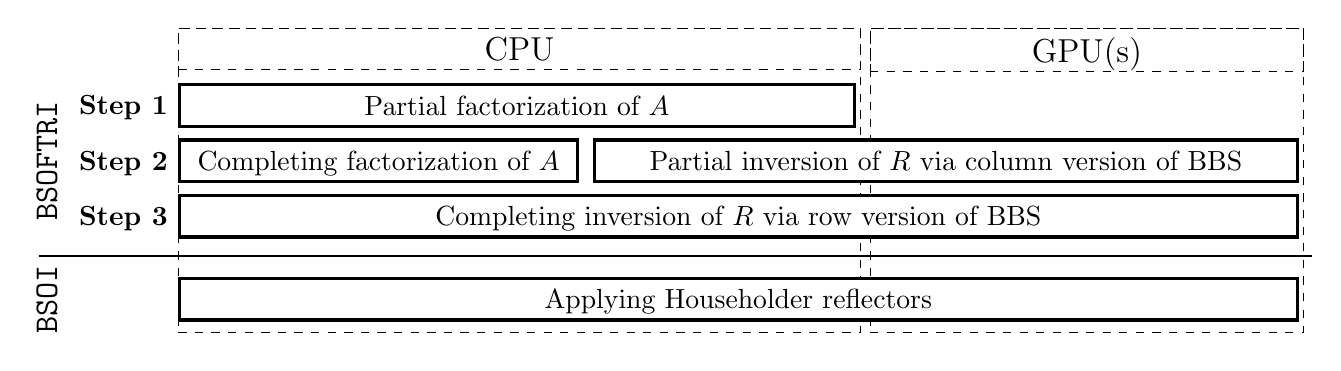
\begin{tikzpicture}[>=latex,text depth=0.0ex]

  \tikzstyle{algBlockStyle}  = [rectangle,fill=white,very thick,inner sep=2pt,minimum height=1.5em,draw,anchor=north west,text centered,]

  \node[text width=24em,minimum height=11em,anchor=north west,dashed,draw] at (0,2em) {};
  \node[text width=24em,anchor=north west,text centered,dashed,draw] at (0,2em) {\large CPU};
  \node[text width=15em,minimum height=11em,anchor=north west,dashed,draw] at (25em,2em) {};
  \node[text width=15em,anchor=north west,text centered,dashed,draw] at (25em,2em) {\large GPU(s)};
  % . 
  \node[algBlockStyle,text width=24em] (BSOFTRI1) {%
    Partial factorization of $A$
    % (without updating the last block column)
  };
  \node [anchor=east] at (BSOFTRI1.west) {{\bf Step 1}};

  \node[algBlockStyle,text width=14em] (BSOFTRI2) at (0,-2em) {%
    Completing factorization of $A$
  };
  \node[algBlockStyle,text width=25em] at (15em,-2em) {
    Partial inversion of $R$ via column version of BBS
  };
  \node [anchor=east] at (BSOFTRI2.west) {{\bf Step 2}};

  \node[algBlockStyle,text width=40em] (BSOFTRI3) at (0em,-4em) {
    Completing inversion of $R$ via row version of BBS
  };
  \node [anchor=east] at (BSOFTRI3.west) {{\bf Step 3}};
  
  \node[algBlockStyle,text width=40em] (BSOI) at (0em,-7em) {
    Applying Householder reflectors
  };

  \draw (-5em,-6.25em) -- (41em,-6.25em);
  \path (BSOFTRI2.west) +(-4em,0) node [anchor=south,rotate=90] {\large \Bsoftri};
  \path (BSOI.west) +(-4em,0) node [anchor=south,rotate=90] {\large \Bsoi};

\end{tikzpicture}

  }
  \caption{Framework of the BSOFI
    adopted to execution on hybrid CPU+GPU platforms.%
    \label{fig:BSOFI_HostDevice}}
\end{figure}
To overcome the lack of parallelism and {\tt DGEMM} operations 
in the factorization phase,  % (Fig.\,\ref{alg:BSOF})
we modify the basic BSOFI algorithm 
by merging the first two phases -- 
factorization of $H$ and inversion of factor $R$ -- 
in a single factorization/inversion algorithm \Bsoftri. 
Hence, in the \Bsoftri,
factorization is a part of computation process which
utilizes both host and devices in parallel.
% On the contrary, 
% MMM dominate over all other kernels 
% in applying Householder reflectors phase.
% Thus, major modification of \Bsoi consists in 
% balanced work-load distribution between host and accelerators.

The merged factorization/inversion phase consists of three steps.
At the first step, 
we perform partial factorization of input $p$-cyclic matrix $H$ 
on the host, where we run $l_F$ loop iterations 
of \Bsof algorithm (see Fig.\,\ref{alg:BSOF}).
% without updating the last block column.
This step is aimed at preparing columns of $R$ for further inversion and 
avoiding idles related to synchronizing concurrent threads in the next step.
Since the optimal number of iterations $l_F$ is usually relatively small,
this step does not influence the overall performance of the algorithm much.
% absence of $p \gg 1$
% Although this step does not involve GPUs in the computation process,
% as shown in the next paragraph, it 
% and hence 
At the second step, 
we fork the computational process on two asynchronous threads.
The first thread completes factorization on CPU,  
whereas the second one computes upper left corner of matrix $R^{-1}$
performing iterations of the column-wise inversion 
algorithm {\tt BSTRI\_CV} (see Fig.\,\ref{alg:BSTRI_CV}).
% without updating the last column panel.
Once the SOF is completed, 
we join both threads and proceed to the third step,
where we continue computing $R^{-1}$
via row version of the BBS algorithm {\tt BSTRI\_RV} (see Fig.\,\ref{alg:BSTRI_RV})
omitting treatment of the $j_F$ already inverted blocks columns of $R^{-1}$.
Switching from column-wise to row-wise inversion algorithm 
reduces computational complexity of \Bsoftri 
compared to the algorithm which uses only column version of BBS.

Depending on the ratio between multicores and device performance and the value of $p$, 
we make a decision on the need for processing 
the last column panel in \Bsoftri inversion thread.
If device performance is insufficient to invert 
more than first $p-2$ column panels of $R$
while $H$ is factorizing, 
we postpone processing the last column panel 
in order to avoid doubling of computational costs 
introduced by the original column version of BBS shown in Fig.\,\ref{alg:BSTRI_CV}
(see table\,\ref{tab:developed_routines_complexity}).

In order to minimize data transfers from host to device 
in \Bsoftri algorithm,
we employ devices in computing only those blocks of $R^{-1}$,
which correspond to the zero blocks of $R$. 
% whereas the host is involved in computing blocks of $R^{-1}$,
% corresponding to both zero and non-zero blocks of $R$. 
The workload distribution between CPU and GPU(s) is 
controlled by parameters $l_j$ and $l_i$ respectively
as illustrated in Fig.\,\ref{fig:BSTRI_CV_HostDevice_workload} and \ref{fig:BSTRI_RV_HostDevice_workload}.

\begin{figure}[t]%[thb]
  \centering
  % \begin{subfigure}[t]{0.59\linewidth}
  %% \subfloat[{\tt BSTRI\_CV} \label{fig:BSTRI_CV_HostDevice_workload}]{%[Column Version]
  %%   \scalebox{0.59}{  \begin{tikzpicture}[>=latex,text depth=0.0ex]

    \begin{scope}[xshift=-5*\SizeMatrBlock,yshift=-5*\SizeMatrBlock]
      \node[matrix,row sep=1pt,column sep=1pt,very thick,rectangle,matrix anchor=a1j.north east] (XinputBottom) {
        &\annotCElem{j-1}&\annotCElem{j}\\
        \annotRElem{1}&\osFrame{R}{1j-1}&\labelElem{RonGPU1}\zsFrame{R}{1j}\\
        &\node{$\vdots$};&\node{$\vdots$};\\
        \annotRElem{l_j}&\osFrame{R}{l_j,j-1}&\labelElem{RonGPUn}\zsFrame{R}{l_j,j}\\
        \annotRElem{l_j+1}&\osFrame{R}{l_j+1,j-1}&\labelElem{RonCPU1}\zsFrame{R}{l_j+1,j}\\
        &\node{$\vdots$};&\node{$\vdots$};\\
        \annotRElem{j-2}&\osFrame{R}{j-2,j-1}&\labelElem{RonCPUzeron}\zsFrame{R}{j-2,j}\\
        \annotRElem{j-1}&\otFrame{R}{j-2,j-1}&\isFrame{R}{}\\
        \annotRElem{j}&\zsFrame{R}{j,j-1}&\labelElem{RonCPUn}\itFrame{R}{jj}\\
      };
    \end{scope}
    \vertann[1.5em]{RonGPU1}{RonGPUn}{\scriptsize $l_j$}
    \vertann[3em]{RonGPU1}{RonGPUn}{GPU(s)}
    \vertann[1.5em]{RonCPU1}{RonCPUzeron}{\scriptsize $j-l_j-2$}
    \vertann[3em]{RonCPU1}{RonCPUn}{CPU}
  \end{tikzpicture}
}}
  %% \subfloat[{\tt BSTRI\_RV}\label{fig:BSTRI_RV_HostDevice_workload}]{%[Row Version]
  %%   \scalebox{0.59}{\begin{tikzpicture}[>=latex,text depth=0.0ex]

  \begin{scope}[xshift=-5*\SizeMatrBlock,yshift=-5*\SizeMatrBlock]
    \node[matrix,row sep=1pt,column sep=1pt,very thick,rectangle] (XinputBottom) {
      \annotRElem{i}
      &\labelElem{RonCPU1}\itFrame{R}{ii}
      &\isFrame{R}{i,i+1}
      &\labelElem{RonCPUzero1}\zsFrame{R}{i,i+2}
      &[0.5em]\node{$\cdots$};[0.5em]
      &\labelElem{RonCPUzeron}\zsFrame{R}{i,k}
      &\labelElem{RonGPU1}\zsFrame{R}{i,k+1}
      &\node{$\cdots$};
      &\labelElem{RonGPUn}\zsFrame{R}{i,p-1}
      &\labelElem{RonCPUlast}\isFrame{R}{ip}\\
      % 
      &\zsFrame{R}{i-1,i}
      &\otFrame{R}{i-1,i+1}
      &\osFrame{R}{i-1,i+2}
      &[0.5em]\node{$\cdots$};[0.5em]
      &\osFrame{R}{i-1,k}
      &\osFrame{R}{i-1,k+1}
      &\node{$\cdots$};
      &\osFrame{R}{i-1,p-1}
      &\osFrame{R}{i-1,p}\\
      % 
      &\annotCElem{i}&\annotCElem{i+1}&\annotCElem{i+2}&
      &\annotCElem{p-l_i-1}&\annotCElem{p-l_i}&
      &\annotCElem{p-1}&\annotCElem{p}\\
    };
  \end{scope}
  \horizann[1.em]{RonGPU1}{RonGPUn}{\scriptsize $l_i$}
  \horizann[2.5em]{RonGPU1}{RonGPUn}{GPU(s)}
  \horizann[1.em]{RonCPUzero1}{RonCPUzeron}{\scriptsize $p-i-l_i-2$}
  \horizann[2.5em]{RonCPU1}{RonCPUzeron}{CPU}%{$\cdot$}
  \lhorizann[2.5em]{RonCPUlast}{RonCPUlast}{CPU}

  % \node at (a) {CPU};
\end{tikzpicture}
}}
  %% \subfloat[{\tt BSOI\_Qk}, if \\$l_k + k \leq p$ \label{fig:BSOI_Qk_HostDevice_workload1}]{
  %%   \scalebox{0.59}{  \begin{tikzpicture}[>=latex,text depth=0.0ex]

    \begin{scope}[xshift=-5*\SizeMatrBlock,yshift=-5*\SizeMatrBlock]
      \node[matrix,row sep=1pt,column sep=1pt,very thick,rectangle] (XinputBottom) {
        &\annotCElem{k}&\annotCElem{k+1}\\
        \annotRElem{1}&\isFrame{X}{1k}&\labelElem{XonCPU1}\osFrame{X}{1,k+1}\\
        &\node{$\vdots$};&\node{$\vdots$};\\
        \annotRElem{k-1}&\isFrame{X}{k-1,k}&\osFrame{X}{k-1,k+1}\\
        \annotRElem{k}&\itFrame{X}{k,k}&\labelElem{XonCPUk}\osFrame{X}{k,k+1}\\
        \annotRElem{k+1}&\zsFrame{X}{}&\labelElem{XonCPU1low}\osFrame{X}{}\\
        &&\node{$\vdots$};\\
        \annotRElem{P-l_k}&\zsFrame{X}{}&\labelElem{XonCPUn}\osFrame{X}{}\\
        \annotRElem{P-l_k+1}&\zsFrame{X}{}&\labelElem{XonGPU1}\osFrame{X}{}\\
        &\node{$\vdots$};&\node{$\vdots$};\\
        \annotRElem{P}&\zsFrame{X}{}&\labelElem{XonGPUn}\osFrame{X}{}\\
      };
    \end{scope}
    \vertann[1.5em]{XonCPU1}{XonCPUk}{\scriptsize $k$}
    \vertann[1.5em]{XonCPU1low}{XonCPUn}{\scriptsize $P-k-l_k$}
    \vertann[3em]{XonCPU1}{XonCPUn}{CPU}
    \vertann[1.5em]{XonGPU1}{XonGPUn}{\scriptsize $l_k$}
    \vertann[3em]{XonGPU1}{XonGPUn}{GPU(s)}
  \end{tikzpicture}
}}
  %% \subfloat[{\tt BSOI\_Qk}, if \\$l_k + k > p$ \label{fig:BSOI_Qk_HostDevice_workload2}]{
  %%   \scalebox{0.59}{  \begin{tikzpicture}[>=latex,text depth=0.0ex]

    \begin{scope}[xshift=-5*\SizeMatrBlock,yshift=-5*\SizeMatrBlock]
      \node[matrix,row sep=1pt,column sep=1pt,very thick,rectangle] (XinputBottom) {
        &\annotCElem{k}&\annotCElem{k+1}\\
        \annotRElem{1}&\isFrame{X}{}&\labelElem{XonCPU1}\osFrame{X}{}\\
        &\node{$\vdots$};&\node{$\vdots$};\\
        \annotRElem{P-l_k}&\isFrame{X}{}&\labelElem{XonCPUn}\osFrame{X}{}\\
        \annotRElem{P-l_k+1}&\isFrame{X}{}&\labelElem{XonGPU1}\osFrame{X}{}\\
        &\node{$\vdots$};&\node{$\vdots$};\\
        \annotRElem{k-1}&\isFrame{X}{}&\osFrame{X}{}\\
        \annotRElem{k}&\itFrame{X}{1j}&\labelElem{XonGPUk}\osFrame{X}{}\\
        \annotRElem{k+1}&\zsFrame{X}{}&\labelElem{XonGPU1low}\osFrame{X}{}\\
        &\node{$\vdots$};&\node{$\vdots$};\\
        \annotRElem{P}&\zsFrame{X}{}&\labelElem{XonGPUn}\osFrame{X}{}\\
      };
    \end{scope}
    \vertann[1.5em]{XonCPU1}{XonCPUn}{\scriptsize $P-l_k$}
    \vertann[3em]{XonCPU1}{XonCPUn}{CPU}
    \vertann[1.5em]{XonGPU1}{XonGPUk}{\scriptsize $k+l_k-P$}
    \vertann[1.5em]{XonGPU1low}{XonGPUn}{\scriptsize $P-k$}
    \vertann[3em]{XonGPU1}{XonGPUn}{GPU(s)}
  \end{tikzpicture}
}}

  \begin{subfigure}[t]{0.2\linewidth}
    \scalebox{0.59}{  \begin{tikzpicture}[>=latex,text depth=0.0ex]

    \begin{scope}[xshift=-5*\SizeMatrBlock,yshift=-5*\SizeMatrBlock]
      \node[matrix,row sep=1pt,column sep=1pt,very thick,rectangle,matrix anchor=a1j.north east] (XinputBottom) {
        &\annotCElem{j-1}&\annotCElem{j}\\
        \annotRElem{1}&\osFrame{R}{1j-1}&\labelElem{RonGPU1}\zsFrame{R}{1j}\\
        &\node{$\vdots$};&\node{$\vdots$};\\
        \annotRElem{l_j}&\osFrame{R}{l_j,j-1}&\labelElem{RonGPUn}\zsFrame{R}{l_j,j}\\
        \annotRElem{l_j+1}&\osFrame{R}{l_j+1,j-1}&\labelElem{RonCPU1}\zsFrame{R}{l_j+1,j}\\
        &\node{$\vdots$};&\node{$\vdots$};\\
        \annotRElem{j-2}&\osFrame{R}{j-2,j-1}&\labelElem{RonCPUzeron}\zsFrame{R}{j-2,j}\\
        \annotRElem{j-1}&\otFrame{R}{j-2,j-1}&\isFrame{R}{}\\
        \annotRElem{j}&\zsFrame{R}{j,j-1}&\labelElem{RonCPUn}\itFrame{R}{jj}\\
      };
    \end{scope}
    \vertann[1.5em]{RonGPU1}{RonGPUn}{\scriptsize $l_j$}
    \vertann[3em]{RonGPU1}{RonGPUn}{GPU(s)}
    \vertann[1.5em]{RonCPU1}{RonCPUzeron}{\scriptsize $j-l_j-2$}
    \vertann[3em]{RonCPU1}{RonCPUn}{CPU}
  \end{tikzpicture}
}
    \caption{{\tt BSTRI\_CV} \label{fig:BSTRI_CV_HostDevice_workload}}
  \end{subfigure}
  \begin{subfigure}[t]{0.4\linewidth}
    \scalebox{0.59}{\begin{tikzpicture}[>=latex,text depth=0.0ex]

  \begin{scope}[xshift=-5*\SizeMatrBlock,yshift=-5*\SizeMatrBlock]
    \node[matrix,row sep=1pt,column sep=1pt,very thick,rectangle] (XinputBottom) {
      \annotRElem{i}
      &\labelElem{RonCPU1}\itFrame{R}{ii}
      &\isFrame{R}{i,i+1}
      &\labelElem{RonCPUzero1}\zsFrame{R}{i,i+2}
      &[0.5em]\node{$\cdots$};[0.5em]
      &\labelElem{RonCPUzeron}\zsFrame{R}{i,k}
      &\labelElem{RonGPU1}\zsFrame{R}{i,k+1}
      &\node{$\cdots$};
      &\labelElem{RonGPUn}\zsFrame{R}{i,p-1}
      &\labelElem{RonCPUlast}\isFrame{R}{ip}\\
      % 
      &\zsFrame{R}{i-1,i}
      &\otFrame{R}{i-1,i+1}
      &\osFrame{R}{i-1,i+2}
      &[0.5em]\node{$\cdots$};[0.5em]
      &\osFrame{R}{i-1,k}
      &\osFrame{R}{i-1,k+1}
      &\node{$\cdots$};
      &\osFrame{R}{i-1,p-1}
      &\osFrame{R}{i-1,p}\\
      % 
      &\annotCElem{i}&\annotCElem{i+1}&\annotCElem{i+2}&
      &\annotCElem{p-l_i-1}&\annotCElem{p-l_i}&
      &\annotCElem{p-1}&\annotCElem{p}\\
    };
  \end{scope}
  \horizann[1.em]{RonGPU1}{RonGPUn}{\scriptsize $l_i$}
  \horizann[2.5em]{RonGPU1}{RonGPUn}{GPU(s)}
  \horizann[1.em]{RonCPUzero1}{RonCPUzeron}{\scriptsize $p-i-l_i-2$}
  \horizann[2.5em]{RonCPU1}{RonCPUzeron}{CPU}%{$\cdot$}
  \lhorizann[2.5em]{RonCPUlast}{RonCPUlast}{CPU}

  % \node at (a) {CPU};
\end{tikzpicture}
}
    \caption{{\tt BSTRI\_RV}\label{fig:BSTRI_RV_HostDevice_workload}}
  \end{subfigure}
  \begin{subfigure}[t]{0.17\linewidth}
    \scalebox{0.59}{  \begin{tikzpicture}[>=latex,text depth=0.0ex]

    \begin{scope}[xshift=-5*\SizeMatrBlock,yshift=-5*\SizeMatrBlock]
      \node[matrix,row sep=1pt,column sep=1pt,very thick,rectangle] (XinputBottom) {
        &\annotCElem{k}&\annotCElem{k+1}\\
        \annotRElem{1}&\isFrame{X}{1k}&\labelElem{XonCPU1}\osFrame{X}{1,k+1}\\
        &\node{$\vdots$};&\node{$\vdots$};\\
        \annotRElem{k-1}&\isFrame{X}{k-1,k}&\osFrame{X}{k-1,k+1}\\
        \annotRElem{k}&\itFrame{X}{k,k}&\labelElem{XonCPUk}\osFrame{X}{k,k+1}\\
        \annotRElem{k+1}&\zsFrame{X}{}&\labelElem{XonCPU1low}\osFrame{X}{}\\
        &&\node{$\vdots$};\\
        \annotRElem{P-l_k}&\zsFrame{X}{}&\labelElem{XonCPUn}\osFrame{X}{}\\
        \annotRElem{P-l_k+1}&\zsFrame{X}{}&\labelElem{XonGPU1}\osFrame{X}{}\\
        &\node{$\vdots$};&\node{$\vdots$};\\
        \annotRElem{P}&\zsFrame{X}{}&\labelElem{XonGPUn}\osFrame{X}{}\\
      };
    \end{scope}
    \vertann[1.5em]{XonCPU1}{XonCPUk}{\scriptsize $k$}
    \vertann[1.5em]{XonCPU1low}{XonCPUn}{\scriptsize $P-k-l_k$}
    \vertann[3em]{XonCPU1}{XonCPUn}{CPU}
    \vertann[1.5em]{XonGPU1}{XonGPUn}{\scriptsize $l_k$}
    \vertann[3em]{XonGPU1}{XonGPUn}{GPU(s)}
  \end{tikzpicture}
}
    \caption{{\tt BSOI\_Qk}, if \\$l_k + k \leq p$ \label{fig:BSOI_Qk_HostDevice_workload1}}
  \end{subfigure}
  \begin{subfigure}[t]{0.17\linewidth}
    \scalebox{0.59}{  \begin{tikzpicture}[>=latex,text depth=0.0ex]

    \begin{scope}[xshift=-5*\SizeMatrBlock,yshift=-5*\SizeMatrBlock]
      \node[matrix,row sep=1pt,column sep=1pt,very thick,rectangle] (XinputBottom) {
        &\annotCElem{k}&\annotCElem{k+1}\\
        \annotRElem{1}&\isFrame{X}{}&\labelElem{XonCPU1}\osFrame{X}{}\\
        &\node{$\vdots$};&\node{$\vdots$};\\
        \annotRElem{P-l_k}&\isFrame{X}{}&\labelElem{XonCPUn}\osFrame{X}{}\\
        \annotRElem{P-l_k+1}&\isFrame{X}{}&\labelElem{XonGPU1}\osFrame{X}{}\\
        &\node{$\vdots$};&\node{$\vdots$};\\
        \annotRElem{k-1}&\isFrame{X}{}&\osFrame{X}{}\\
        \annotRElem{k}&\itFrame{X}{1j}&\labelElem{XonGPUk}\osFrame{X}{}\\
        \annotRElem{k+1}&\zsFrame{X}{}&\labelElem{XonGPU1low}\osFrame{X}{}\\
        &\node{$\vdots$};&\node{$\vdots$};\\
        \annotRElem{P}&\zsFrame{X}{}&\labelElem{XonGPUn}\osFrame{X}{}\\
      };
    \end{scope}
    \vertann[1.5em]{XonCPU1}{XonCPUn}{\scriptsize $P-l_k$}
    \vertann[3em]{XonCPU1}{XonCPUn}{CPU}
    \vertann[1.5em]{XonGPU1}{XonGPUk}{\scriptsize $k+l_k-P$}
    \vertann[1.5em]{XonGPU1low}{XonGPUn}{\scriptsize $P-k$}
    \vertann[3em]{XonGPU1}{XonGPUn}{GPU(s)}
  \end{tikzpicture}
}
    \caption{{\tt BSOI\_Qk}, if \\$l_k + k > p$ \label{fig:BSOI_Qk_HostDevice_workload2}}
  \end{subfigure}

  \caption[]{Workload distribution between host and device(s) 
    while processing 
    $j$th block column and $i$th block row of $R^{-1}$ (a,b) 
    and applying $Q_k^T$ to $R^{-1}$ (c,d).\footnotemark}
  \label{fig:HostDevice_workload}
\end{figure}
\footnotetext{
  White -- zero blocks, 
  light gray -- input non-zero blocks, 
  dark gray -- blocks processed (partially or fully) 
  in the preceding iteration.
  Irrelevant zero blocks are omitted.}

In the phase of applying Householder reflectors to $R^{-1}$,
we update block column pairs by means of 
explicit reconstruction of matrices $Q^{(k)}$
and the scheme similar to the algorithm shown in Fig.\,\ref{alg:BSOI_Qk}.
In this way, we replace {\tt DORMQR} calls for applying reflectors to column panels 
% which apply Householder reflectors, 
in favor of more efficient {\tt DGEMM} calls
under the small computational overhead.
The upper parts of block columns are updated on the host, 
whereas devices are used to update lower parts. 
Since the lower part of $R^{-1}$ has more zero blocks,
this approach requires less data transfers from CPU to GPUs.
In order to avoid physical data transfers inside devices,
we store block columns of the input matrix $W$ in the reversed order 
with respect to the natural order of columns in matrix $X$. 
Namely, the $(k+1)$th block column of $X$ 
corresponds to ${W}_{:,1}$ and 
the $k$th block column of $X$ 
corresponds to ${W}_{:,2}$.
Herewith we use the following equality to update column pairs on device 
\begin{equation}
  \label{BSOI_device_update}
    X_{p-l_k:p,k:k+1}   Q^{{(k)}T} = 
    \begin{bmatrix}
      X_{p-l_k:p,k+1} & X_{p-l_k:p,k}
    \end{bmatrix} 
    \begin{bmatrix}
      Q^{(k)}_{1:2,2} & Q^{(k)}_{1:2,1}
    \end{bmatrix}^T  
    % \begin{bmatrix}
    %   Q^{(k)}_{12} & Q^{(k)}_{11}\\
    %   Q^{(k)}_{22} & Q^{(k)}_{21}
    % \end{bmatrix}^T  
    %= X_{p-l_k:p,k+1}  Q^{(k)T}_{1:2,2} + X_{p-l_k:p,k}  Q^{(k)T}_{1:2,1}.
\end{equation}

The workload distribution between host and device
is controlled by % parameters
$l_k$. 
% There are two possible situations shown in Fig.\,\ref{fig:BSOI_Qk_HostDevice_workload1}.
If $l_k + k \leq p$ (Fig.\,\ref{fig:BSOI_Qk_HostDevice_workload1}),
then $X_{p-l_k:p,k}=0$,
and hence device does not require sub-matrix $Q^{(k)}_{1:2,1}$
to compute update according to (\ref{BSOI_device_update}).
In contrast,
if $l_k + k > p$ (Fig.\,\ref{fig:BSOI_Qk_HostDevice_workload1}),
whole matrix $Q^{(k)}$ and non-zero blocks of $k$th column panel of $X$
should be sent from host to device for further processing.
For more details on the algorithm presented in this paragraph,
see~\cite{GogolenkoBai13}.

% \subsection{Employing multiple GPUs}
% \label{sec:multi-GPU}
% To improve the load balancing if several GPUs are used,  
% we use the round-robin tournament for distribution 
% of matrix blocks between devices. 
% E.g., while inverting $R$ via column version of BBS,
% the $k$th GPU is responsible for $k$th, $(m + k)$th, 
% $(2m+k)$th, etc rows, where $m$ is a total number of utilized GPUs.
% In addition, we adjust formulae\,(\ref{eq:l_i})--(\ref{eq:l_k})
% for computing load balancing parameters, 
% using simple replacement of 
% % GPU performance  $P^{GPU}$ by $m P^{GPU}$ 
% % in the expressions for $\kappa_R$, $\kappa_C$ and $\kappa_Q$.
% $\kappa_R$, $\kappa_C$, and $\kappa_Q$ 
% by $\kappa_R/m$, $\kappa_C/m$, and $\kappa_Q/m$ respectively.


\paragraph{Performance modelling and load balancing.} \label{sec:load_balancing_parameters}

The parameters $l_i$, $l_j$, $l_k$ and $l_F$ 
introduced in the previous paragraph,
control workload distribution between host and devices, 
and play a crucial role in performance tuning.
The following text is an excerpt of results related to 
% the load balancing by
choosing above-mentioned parameters and performance modelling.
These results are based on the following assumptions: 
\begin{inparaenum}[(i)]
\item the elapsed time for 
  multiplying $mn$-by-$n$ and $kn$-by-$n$ matrices
  is nearly $mk$ times more than the wall time for computing the product
  of two $n$-by-$n$ matrices;
% $T^{CR}_{\texttt{DGEMM(m*n,k*n,n)}}\approx m k{\cdot}T^{CR}_{\texttt{DGEMM(n,n,n)}}$
\item the performance of numerical kernel
  is roughly proportional to the number of CPU cores utilized in its computing.
\end{inparaenum}
These assumptions are consistent with benchmarking results 
for moderate and large values of $n$~\cite{GogolenkoBai13}.
For more details and derivation of formulae, we refer to~\cite{GogolenkoBai13}.

The formulae presented below use the following notation for time measures.
$T^{\rm cr}_{\texttt{R(P)}}$ denotes the wall time 
for BLAS and LAPACK routines {\tt R} with a tuple of parameters {\tt P}
on the computational resource CPU or GPU, respectively.
E.g., $T^{\rm cpu}_{\texttt{DGEMM(m,n,k)}}$ is an elapsed time for 
computing a product of $m$-by-$k$ and $k$-by-$n$ matrices
by means of the routine $\texttt{DGEMM}$ on the CPU.
We alias the routines for copying rectangular matrices to and from GPU 
with {\tt SET} and {\tt GET} respectively.
We use braces if 
these data exchange operations can be executed algorithmically 
in parallel with some numerical kernel(s).
I.e., $\{T_{\texttt{DGEMM(n,n,n)}}^{\rm gpu},T^{\rm gpu}_{\texttt{GET(n,n)}}\}$ 
is equal to 
$\max\{T_{\texttt{DGEMM(n,n,n)}}^{\rm gpu},T^{\rm gpu}_{\texttt{GET(n,n)}}\}$ 
if copying is asynchronous and implemented 
via {\tt cublasGetMatrixAsync}, 
and $T_{\texttt{DGEMM(n,n,n)}}^{\rm gpu}+T^{\rm gpu}_{\texttt{GET(n,n)}}$ 
if synchronous routine {\tt cublasGetMatrix} is used.
% In addition, $\eta_I$ and $\eta_F$ denote fractions 
% of host resources assigned to 
% column-wise inversion thread and factorization thread 
% in the merged factorization/inversion phase
% respectively.

The optimal values of the parameters $l_j$, $l_i$, and $l_k$ 
correspond to the situation 
if the elapsed time of processing assigned kernels
on both host and devices are roughly the same in each iteration. 
These conditions result in the following approximations 
\begin{align}
% \begin{equation}
  \label{eq:l_j}
  l_j \approx \frac{1}{1 + \kappa_C} \left(j + c_j \right)
  , \quad %\label{eq:l_i}
  l_i \approx \frac{1}{1 + \kappa_R} \left( p-\min\{i,j_F\}+1 + c_i \right), 
  \\
% \end{equation}
% \begin{equation}
  \label{eq:l_k}
    l_k \approx 
    \begin{cases}
        \displaystyle \frac{1}{1 + \kappa_Q} \left( p+k + 2 +c'_k - c''_k\right),
      & \mbox{if } k \leq \displaystyle \frac{ \kappa_{Q} p -2 - c'_{k}}{\kappa_{Q} + 2},\\ %k_{s}
        \displaystyle \frac{1}{1 + \kappa_Q} \left(p  + \frac{\kappa_Q}{2}(p-k) + 1 + c'_k/2 - c''_k\right),
      & \mbox{if } k > \displaystyle \frac{ \kappa_{Q} p -2 - c'_{k}}{\kappa_{Q} + 2}, %k_{s}
    \end{cases}
% \end{equation}
\end{align}
where 
\begin{align*}
  \kappa_C =& \frac{\{T_{\texttt{DGEMM(n,n,n)}}^{\rm gpu},T^{\rm gpu}_{\texttt{GET(n,n)}}\}}{T^{\rm cpu}_{\texttt{DGEMM(n,n,n)}} / (1 + \eta)} 
  % = \frac{P^{CPU}_{\square}}{\eta_I P^{GPU}_{\square\gets}}
  , \;
  c_j = 2 \frac{T^{\rm cpu}_{\texttt{DTRTRI(n)}} + 2 T^{\rm cpu}_{\texttt{DTRMM(n,n)}}}{2 T^{\rm cpu}_{\texttt{DGEMM(n,n,n)}}} - 1 > \frac{1}{6}
  ,\;
  \\
  \kappa_R =& \frac{\{T_{\texttt{DGEMM(n,n,n)}}^{\rm gpu},T^{\rm gpu}_{\texttt{GET(n,n)}}\}}{T^{\rm cpu}_{\texttt{DGEMM(n,n,n)}}} 
  % = \frac{P^{CPU}_{\square}}{P^{GPU}_{\square\gets}}
  , \;
  c_i = 
  2 \frac{T^{\rm cpu}_{\texttt{DTRTRI(n)}} + 3T^{\rm cpu}_{\texttt{DTRMM(n,n)}}}{2 T^{\rm cpu}_{\texttt{DGEMM(n,n,n)}}} - 2 > -\frac{1}{3},
  \\
  \kappa_Q  =& \frac{\{T_{\texttt{DGEMM(2*n,n,n)}}^{\rm gpu},T^{\rm gpu}_{\texttt{GET(n,n)}}\}}{T^{\rm cpu}_{\texttt{DGEMM(2*n,n,n)}}} 
  % = \frac{P^{CPU}_{\square}}{P^{GPU}_{\square\frac{\rightleftharpoons}{2}}}
  , \,
  c'_k  = \frac{T^{\rm cpu}_\texttt{DORGQR(2*n,2*n,n)}}{T^{\rm cpu}_\texttt{DGEMM(2*n,n,n)}} - 2 > \frac{1}{3}
  % c'_k  = \frac{5}{2}\frac{T^{CPU}_\texttt{DORGQR(2*n,2*n,n)}}{5 T^{CPU}_\texttt{DGEMM(n,n,n)}} - 2 > \frac{1}{3}
  , \,
  c''_k = {%\kappa_Q 
    \frac{T^{\rm gpu}_{\texttt{SET(n,n)}}}{%\{T_{\texttt{DGEMM(2*n,n,n)}}^{GPU},T^{GPU}_{\texttt{GET(n,n)}}\}
    T_{\texttt{DGEMM(2*n,n,n)}}^{\rm cpu}}}
  ,
\end{align*}
$\eta$ is a ratio between the number of cores involved in factorization of $H$
and the number of cores involved in inversion of $R$ in the second step of \Bsoftri 
(e.g., the typical values of $\eta$ for single hexa-core are $3:3$, $4:2$, or $5:1$).

In order to reduce idle time 
related to % on
the synchronization of parallel threads 
in the merged factorization/inversion phase, 
the total elapsed time for inversion of the first $j_F$ columns % on $1/(1 + \eta)$, 
should be less than 
the elapsed time for performing $j_F-l_F$ factorization steps.
This condition leads to the following lower bound for $l_F$
\begin{equation}
  \label{eq:l_F}
  l_{F}(\delta) \ge
  \frac{1}{2} - c_{j} + \frac{\delta \eta}{10 \beta_F } 
  \left( c_{j}^{2} + c_{j}  - \frac{1}{4} \right) + \frac{5 \beta_F }{2 \delta \eta}
  , \,
  % \beta_F  = \frac{T^{CPU}_{\texttt{DGEQRF(2*n,n)}} + T^{CPU}_{\texttt{DORMQR(% 'R','N',
  %       2*n,n,n)}}}{5 T^{CPU}_{\texttt{DGEMM(n,n,n)}}}  
  % ,
\end{equation}
where 
\begin{equation*}
  % c_F = 2 \alpha_F - 1 = 2 \frac{T^{CPU}_{\texttt{DTRTRI(2n)}}}{2 T^{CPU}_{\texttt{DGEMM(n,n,n)}}} - 1,\;
  \beta_F  = \frac{T^{\rm cpu}_{\texttt{DGEQRF(2*n,n)}} + T^{\rm cpu}_{\texttt{DORMQR('R','N',2*n,n,n)}}}{5 T^{\rm cpu}_{\texttt{DGEMM(n,n,n)}}},
\end{equation*}
$\delta=1$ if the last column panel inversion 
is postponed in the second step of \Bsoftri,
and $\delta=2$ otherwise. 
The latter inequality usually holds true for some $2 \le l_F \le 6$.
If $\delta=1$, $l_F$ and $j_F$ are linked by expression
\begin{equation*}
  \label{eq:l_F2}
  \hat{l}_F(j_F) = p - {\frac{1}{5}\left(\frac{\eta}{\beta_{F} } 
      \left( \frac{1}{2}\frac{\kappa_{C}}{1+\kappa_{C}} 
        \left(j_F^2 + (1+2c_j)j_F  - 4 c_j - 6 \right) % + c_F
        + 1 \right) - 3 p +  10\right) }
  .
\end{equation*}
% \begin{equation}
%   \label{eq:j_F}
%   \begin{split}
%     j_F = \theta
%     {\sqrt{\frac{\beta_{F} }{ \delta \eta} \left(1 + \frac{1}{\kappa_{C}}\right) \left(p - 2\right) }}
%     \quad \text{for some $\sqrt{3} < \theta < 2 \sqrt{2}$.}
%   \end{split}
% \end{equation}
% In other words, $l_F$ should satisfy conditions
Hence, postponed processing of the last column panel in the second step of \Bsoftri 
makes sense only if $l_F(1) > \hat{l}_F(p-2)$
for minimal $l_F$ which satisfies (\ref{eq:l_F}).

Results of the theoretical performance study are summarized in the table\,\ref{tab:Parallel_BSOFTRI_performance}.
For the sake of simplicity, 
the lower order terms are neglected. % not included in the model.
$\theta$ is a decreasing % non-negative
function of $l_F$. 
Its upper bound is $2\sqrt{2}$. 
The lower bound on $\theta$ is $\sqrt{3}$ if $\delta = 1$.
\begin{table}[t]%[thb]
  \caption[]{Performance model of parallel ``host-device'' BSOFI,
where Metric 1 is the number of flops on GPU, 
Metric 2 is  the number of words CPU$\rightleftharpoons$GPU and 
Metric 3 is the number of messages CPU$\rightleftharpoons$GPU. 
\label{tab:Parallel_BSOFTRI_performance}
}
  \begin{tabular}{l|c|c}
    \toprule
    Metric & \Bsoftri & \Bsoi  \\
    \hline\hline %\midrule
    1 
    & $\frac{n^{3} p}{1 + \kappa_{R}} \left( 
      \theta^{2} \beta_F \left( 1 + \frac{\delta - 1 }{\delta \eta} \left( 1 + \frac{1}{\kappa_{C}} \right) \right) 
      + {p + 1 + 2 c_{i}} \right)$
    % & $\frac{6 n^{3} p^{2}}{1 + \kappa_{Q}}$  \\
    & $\frac{2 n^{3} p}{1 + \kappa_{Q}} \left( 3 p + 1 + 2 c'_k - 4 c''_k\right)$\\
    \hline
    2
    & $\frac{n^{2} p}{1 + \kappa_{R}} \frac{1}{2}\left(\frac{\theta^{2} \beta_F }{\delta} + 
      {p + 5 + 2 \kappa_R + 2 c_{i}}\right)$
    & $\frac{n^{2} p^{2}}{1 + \kappa_{Q}} \frac{1}{2} \frac{3 \kappa_{Q} + 4}{ \kappa_{Q} + 2}$ \\
    \hline
    3
    & $2 p + 2(2 - \delta) \theta {\sqrt{\frac{\beta_{F} }{ \delta \eta} \left(1 + \frac{1}{\kappa_{C}}\right) \left(p - 2\right) }}
    + 2 \delta - 12$
    & $2 p-2$ \\
    % \hline
    % \# words CPU$\to$GPU
    % & $\frac{n^{2} p}{ 1 + \kappa_{R}} \left( 2 + \kappa_{R} \right)$
    % & $\frac{n^{2} p}{1 + \kappa_{Q}} \frac{2 \kappa_{Q}^{2} + 13 \kappa_{Q} + 12}{\kappa_{Q} + 2}$\\
    % \hline
    % \# words CPU$\gets$GPU
    % & $\frac{n^{2} p}{1 + \kappa_{R}} \frac{1}{2}\left(\frac{\theta^{2} \beta_F }{\delta} + 
    %   {p + 1 + 2 c_{i}}\right)$
    % & $\frac{n^{2} p^{2}}{1 + \kappa_{Q}} \frac{3 \kappa_{Q} + 4}{2 \kappa_{Q} + 4}$ \\
    % \hline
    % \# messages CPU$\to$GPU
    % & $p + (2 - \delta) \theta {\sqrt{\frac{\beta_{F} }{ \delta \eta} \left(1 + \frac{1}{\kappa_{C}}\right) \left(p - 2\right) }}
    % +\delta - 6$
    % & $p-1$ \\
    % \hline
    % \# messages CPU$\gets$GPU
    % & $p + (2 - \delta) \theta {\sqrt{\frac{\beta_{F} }{ \delta \eta} \left(1 + \frac{1}{\kappa_{C}}\right) \left(p - 2\right) }}
    % +\delta - 6$
    % & $p-1$ \\
    \bottomrule
  \end{tabular}
\end{table}



\section{Experimental results and analysis}
\label{sec:results}

% The purpose of this performance evaluation is to highlight 
% the features of the proposed algorithmic solutions.
% Our experimental study was organized as follows. 
% At first, we explore performance of building blocks 
% in order to illustrate 
% revealing the suboptimal load balancing parameters for hybrid CPU+GPU implementation.
% Here, we turn our particular attention on behaviour of building blocks 
% for matrices $H$ with different 
% values of parameter $n$ from the interval $32 \leq n \leq 2048$.
% Next, we compare performance of our 
% stand-alone CPU implementations with 
% the naive implementations of Gaussian elimination based inversion.
% The purpose of it is to investigate the quality of 
% exploiting structure by our algorithm %!TODO
% comparing with LU factorization based inversion. Finally, 
% we compare performance of all three implementations 
% and show performance results for nodes with single and multiple GPUs
% to highlight benefits of hybrid implementation.
% We refer to the report~\cite{GogolenkoBai13} for more experimental results.

%\textit%%\paragraph
\paragraph{Experimental setup.}
\label{sec:experimental_setup}
%
In order to examine our algorithmic solutions, 
we developed codes for 
stand-alone CPU and GPU processing, 
as well as hybrid CPU+GPU implementation.
Our solvers receive $p$-cyclic matrix $H$ in an unpacked form as input, 
and replace it with its inverse $H^{-1}$ 
by performing in-place inversion. 
% In our {hybrid CPU+GPU implementation}, 
The POSIX threads are used for threading in the second step of \Bsoftri.
For performance data presented below, the codes were compiled with ICC  %@TODO
and linked with \CuBlas, \Magma, and Intel's MKL library. %@TODO
Our codes are publicly available from
\url{https://github.com/SGo-Go/BSOFI}.
% The peak performance of matrix-matrix multiplications (MMM) with \Gemm
% observed on the target platform, is 
% 140\,GFlops for \MKL and 167\,GFlops for \CuBlas. 
% Hence, the gap between peak performance of MMM on GPU and on CPU 
% is relatively small. 
The performance data were collected on a 2-socket Intel Xeon X5670 
coupled with NVIDIA GeForce GTX480 GPU.
Intel Xeon X5670 is a 6-core processor with 2.9GHz clock rate.
GTX480 is a \Cuda-enabled, which implements Fermi architecture, 
and has 15 streaming multiprocessors with 32 \Cuda cores in each.
For multi-GPU studies, we used a multi-GPU Fermi node on the Dirac cluster,
housed at NERSC of Lawrence Berkeley National Laboratory.
This node contains 2 Intel 5530 2.4GHz Quad core Nehalem processors, 
and 4 C1060 NVIDIA Tesla GPUs.

%\textit%%\paragraph
\paragraph{Performance tuning.} %Performance of building blocks and validation of load balancing approach
\label{sec:BB_performance}
%
In order to make our hybrid CPU+GPU codes architecture-aware, 
we perform benchmarking of basic kernels used in the modified SOI algorithm, 
evaluate parameters for (\ref{eq:l_j})--(\ref{eq:l_F}), 
and embed their approximate models into the code.
% The following text illustrates this process 
% using the Dirac's multi-GPU node as a target.
% Benchmarking % the 
% single GPU node gives % the 
% similar results. 
% 
% Due to the influences of data exchanges and 
% difference in the sizes of tasks 
% for which CPUs and GPUs attain maximum MMM performance,
% parameters $\kappa_C$, $\kappa_C$, and $\kappa_Q$ 
% depend dramatically on the block size $n$ if $n$ is small.
Our experiments have shown that 
parameters $\kappa_R$, $\kappa_C$, and $\kappa_Q$ 
depend dramatically on the block size $n$ if $n$ is small, and
this dependence can be sufficiently well
approximated by the first order rational functions. 
% Thus, we approximate $\kappa$-parameters by a piecewise function
% with a constant piece for large values of $n$ and rational for small. 
We obtain parameters of these rational functions 
% on the basis of benchmarks
by Gauss-Markov estimator. 
% using Levenberg-Marquardt algorithm for least squares optimization.
% Fig.\,\ref{fig:kappa_params} shows the fitted $\kappa$-curves
% for the Dirac's multi-GPU node.
% 
The correction parameters $c_i$, $c_j$, $c'_k$, and $c''_k$ %in (\ref{eq:l_j})--(\ref{eq:l_F}) 
% MMM has usually 
% much higher performance than 
% the rest of the kernels involved in the BSOFI algorithm. 
are approximated by descending step-wise functions of $n$.
% rounding benchmarking results to the closest 
At first, we filter curves for these parameters received after benchmarking, % to reduce influence of undesirable impulses
and afterwards round the filtered curves to the closest integers.
% We use Hann window function for filtering as a default option.
The same approach is used to build a step-wise approximation for parameter $l_F$.
% Fig.\,\ref{fig:step_wise_params} illustrates resulting approximations 
% for the Dirac's multi-GPU node.

%\textit%%\paragraph
\paragraph{Benchmarking results.}\label{sec:benchmarking}
%
% \paragraph{Comparison with  LU based inversion}\label{sec:compare_naive}
%
% Next, we compare performance of our 
% stand-alone CPU implementations with 
% the naive implementations of Gaussian elimination based inversion.
To investigate the quality of exploiting structure by BSOFI algorithm,
% In Fig.\,\ref{fig:speedup_cpu12}, 
we compare performance of our 
CPU implementation with na\"ive BLAS3 LU inversion 
and inversion by multifrontal sparse LU solvers from {\sc UMFPack}. 
Benchmarking shows % The figure illustrates
significant speed-up 
of BSOFI with respect to LU inversion. %if the size of matrix increases.
We observe up to $22\times$ speed-up if $n\times p < 10^4$ and $n \ge 32$. 
The general tendency is an increase of speed-up with a decrease of $n$.

% \begin{figure}[t]%[thb]
%   \centering
%   \includegraphics[width=.45\textwidth]{./figs/pdf/BSOF_BSTRI_BSOI_cpu_12}
%   \caption{Speed-up of the BSOFI with respect to 
%     the LU inversion on two sockets of Intel Xeon X5670.
%     \label{fig:speedup_cpu12}}
% \end{figure}

% \paragraph{Performance of CPU, GPU and hybrid implementations}\label{sec:compare_performance}

Fig.\,\ref{fig:compare_BSOFTRI+BSOI} shows the performance of 
BSOFI codes on different platforms for $N=10240$.
% We use the single GPU node for illustration, 
% and present results for GPU, CPU (1 and 2 sockets) and 
% hybrid CPU+GPU implementations.
\begin{figure}[t]%[thb]
  \centering
  %% \subfloat[Performance of the CPU, GPU and hybrid BSOFI codes\label{fig:compare_BSOFTRI+BSOI}]{
  %%   \includegraphics[width=0.4\textwidth]{./figs/pdf/BSOFI_BSOI_12}}
  %% \subfloat[Performance of the hybrid BSOFI codes\label{fig:perf_hybrid_BSOFTRI_BSOI}]{
  %%   \includegraphics[width=0.4\textwidth]{./figs/pdf/BSOFTRI_BSOI}}

  \begin{subfigure}[t]{0.49\linewidth}
    \includegraphics[width=\textwidth]{./figs/pdf/BSOFI_BSOI_12}
    \caption{Performance of the CPU, GPU and hybrid BSOFI codes\label{fig:compare_BSOFTRI+BSOI}}
  \end{subfigure}
  \begin{subfigure}[t]{0.49\linewidth}
    \includegraphics[width=\textwidth]{./figs/pdf/BSOFTRI_BSOI}
    \caption{Performance of the hybrid BSOFI codes\label{fig:perf_hybrid_BSOFTRI_BSOI}}
  \end{subfigure}
  \caption{Performance of BSOFI on 
    a 2-socket Intel Xeon X5670 coupled with NVIDIA GeForce GTX480 GPU.} 
  \label{fig:performance_BSO}
\end{figure}
%
Hybrid implementation is up to $1.7\times$ faster over the 
best of CPU and GPU codes.
Its peak performance is higher than peak 
performance of \Gemm on CPU 
and is only $1.1\times$ lower than the peak of \Gemm on GPU.
Moreover, 
the difference in performance in the interval $32 \leq n \leq 1024$ 
does not exceed $1.5\times$ for our hybrid CPU+GPU implementation. % , 
% which allows to conclude that this code works quite efficiently for different values of $n$. 
%
Fig.\,\ref{fig:perf_hybrid_BSOFTRI_BSOI} %\ref{fig:perf_hybrid_cpu_512} 
compares 
the performance of CPU+GPU codes for different sizes of $p$-cyclic matrices if $n$ is fixed. 
If $n$ is large, performance of subroutine \Bsoi on the single GPU node 
is two times more in the case of CPU+GPU implementation  
than in the case of pure CPU implementation.
At the same time, 
performance improvements for subroutine \Bsoftri 
are less significant than for \Bsoi.
% Figure~\ref{fig:perf_hybrid} 
% shows
% performance of hybrid CPU+GPU codes for different values of $n$ and $p$. 
If $n \gtrapprox 512$, performance curves are close to each other. 
This is a consequence of reaching maximum performance for {\tt DGEMM}
on both CPU and GPU. 
% \begin{figure}[h]
%   \centering
%   \includegraphics[width=3.4in]{./figs/pdf/BSOFTRI_BSOI}
%   \label{fig:perf_hybrid_BSOFTRI_BSOI}
%   \caption{Performance of the hybrid BSOFI codes 
%     with the size of matrix for different block sizes $n$.}
%   \label{fig:perf_hybrid}
% \end{figure}

More benchmarking results on both single and multi-GPU platforms 
can be found in~\cite{GogolenkoBai13}.

\section{Conclusions and further directions}
\label{sec:conclusions}

We presented serial and parallel algorithms for structured orthogonal inversion
of block $p$-cyclic matrices. % by introducing 
% a number of techniques for high performance computing, 
% such as blocking, batching and load balancing.
We provided a performance model and discussed host-device load balance.
We developed and explored CPU, GPU and hybrid CPU+GPU codes
for in-place inversion of $p$-cyclic matrices. % The key trait of our 
% hybrid CPU+GPU implementation is in 
% using GPUs only for MMMs for better utilization of these devices.
Benchmarking has shown that 
our codes for multicores with GPU accelerators
maintain sustainable performance for different values 
of problem size $n$, and attain up to 90\% of realistic peak performance in 
terms of the operation of the matrix-matrix multiplication. 

There are numerous ways to extend the results presented in this paper.
Since GPUs have a lot in common with Intel MIC architecture, 
it seems natural to verify the approaches
on multicores with MIC accelerators.
% The major bottleneck of the basic SOI algorithm 
% is a lack of parallelism in the orthogonal factorization phase. 
% In this paper, we solved this problem by merging factorization phase 
% with the phase of computing $R^{-1}$.
% An alternative approach is in applying a parallel version 
% of SOF, and then it potentially 
% introduces a new parallelism into the phase of applying Householder reflectors.
% However, implementation of this idea encompasses a large amount of work 
% related to development of batched kernels for the small 
% QR factorization on GPUs.  Although there are some known 
% attempts to develop batched QR factorization codes~\cite{Anderson12}, 
% we are not aware about any actively 
% used numerical software supporting this functionality.
%
Another promising direction is in coupling of 
SOI with inversion based on explicit formulae. 
% As far as explicit formulae for inverse of $p$-cyclic matrices 
% include long chains of matrix-matrix products, 
% explicit inversion algorithms require a computationally expensive 
% stabilized chained matrix-matrix multiplication algorithms
% if $p$ is large, e.g. $p > 10$.  However, if $p$ is relatively small, 
% MMM can be sufficient to attain appropriate results.
% This suggests an inversion approach, 
% where at first we reduce the $p$-cyclic matrix to a smaller one, 
% then use orthogonal inversion method to compute inverse of the reduced matrix, 
% and finally recover elements by means of formulae for explicit inversion.
%
We conclude by mentioning 
that the solutions proposed here can be extended to 
the problems with other block structured matrices such as
block upper Hessenberg matrices. 
This leads us to believe that the BSOFI could be a vital substitute 
to conventional Gaussian elimination based inversion
for broader classes of block structured matrices.
% For example, it is straightforward that the algorithms presented here 
% can be applied for the inversion of 
% multipoint bordered almost block diagonal matrices~\cite{Amodio00}.

\bibliographystyle{splncs03}
\bibliography{bsofi}
\end{document}


